\section{Plot Generation}
Each block that is sent into the PlotGenerator is treated differently depending on what the block label is. 
If the block label is either \textit{Parks} or \textit{Parking}, then the PlotGenerator does not split the block. 
The entire block is turned into a plot and is sent to ParkGenerator or ParkingGenerator respecitvely.
The rest of the block labels are split into n parts, where n depends on the area of the block and some randomness. 

In Figure \ref{fig:plot} and \ref{fig:plot2} are examples of the output for the PlotGenerator.

\begin{figure}[H]
  \centering

  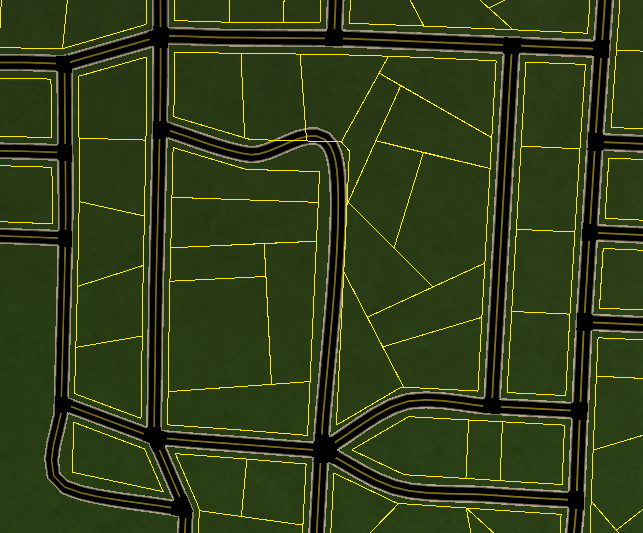
\includegraphics[width=0.8\textwidth]{figure/plot2.png}
  \caption{Close-up of the plot splitting algorithm.}

  \label{fig:plot2}
\end{figure}

\begin{figure}[H]
  \centering

  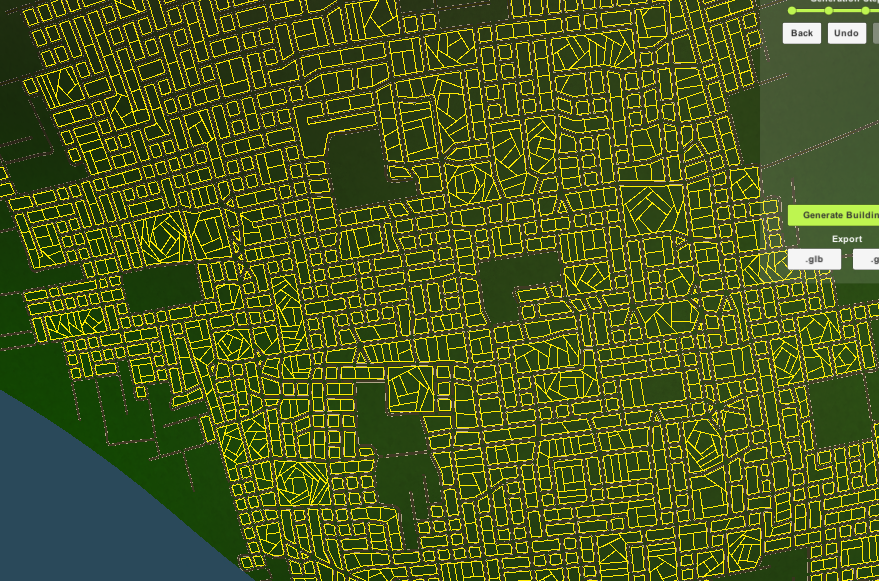
\includegraphics[width=0.8\textwidth]{figure/plot.png}
  \caption{Plot splitting for a city.}

  \label{fig:plot}
\end{figure}

Each plot is assigned a plot label, used to find the correct content generator.
The plot labels are \textit{Manhattan}, \textit{Skyscraper}, \textit{Park}, \textit{Parking}, and \textit{Empty}.
\textit{Manhattan} and \textit{Skyscraper} are two different sub-generators for BuildingGenerator. 
\textit{Park} and \textit{Parking} has ParkGenerator and ParkingGenerator respecitvely.
If the plot label is \textit{Empty}, then no content is generated upon the plot. 
